\documentclass{beamer}
\usepackage{graphicx}
\usepackage{tikz}
\usetikzlibrary{shapes,arrows}
\usepackage{tikz}
%\usecolortheme{seahorse}
  \setbeamertemplate{footline}[page number]
\usepackage{multirow}
\setbeamertemplate{navigation symbols}{}
\setbeamertemplate{frametitle}[default][center]
\setbeamerfont{frametitle}{shape=\scshape}
\usepackage{color}

\usepackage{csquotes}

\usepackage{xcolor}

\usepackage[flushleft]{threeparttable}

{\title{\textsc{Econ 352 - A Real Intertemporal Model with Investment} \\ \tiny (See Williamson Ch. 11)}
\author{Trevor S. Gallen}
\date{}
\begin{document}
\renewcommand*{\inserttotalframenumber}{\pageref{lastframe}}


\setbeamertemplate{caption}{\raggedright\insertcaption\par}

\begin{frame}
\titlepage
\end{frame}

\begin{frame}
\frametitle[alignment=center]{Introduction}
\begin{itemize}
\item We have the intratemporal and intertemporal components of the household's problem
\bigskip
\item Now we'll put them together and build a real intertemporal model with investment
\bigskip
\item This model is at the core of all modern macro, which just adds bells \& whistles (rigidity, search/matching, imperfections, heterogeneity).
\end{itemize}
\end{frame}

\begin{frame}
\frametitle[alignment=center]{Representative Consumer}
\begin{itemize}
\item Representative consumer takes a number of things as \emph{given}, even though they are endogenous in the model:
\smallskip
\begin{itemize}
\item Prices: the real wage now and in the future $w$ and $w'$, and the real interest rate $r$
\smallskip
\item Taxes now and in the future: $T$ and $T'$
\smallskip
\item Firm profits today and tomorrow $\pi$ and $\pi'$
\end{itemize}
\smallskip
\item The representative consume makes five decisions: leisure ($\ell$ and $\ell'$) and consumption (C and $C'$) and investment $S^P$
\end{itemize}
\end{frame}


\begin{frame}
\frametitle[alignment=center]{Representative Consumer}
\begin{itemize}
\item Faces budget constraint today and tomorrow:
$$C+S^P=w(h-\ell)+\pi-T$$
$$C= w'(h'-\ell')+\pi'-T'+(1+r)S^P$$
\item Combining as we have in past chapters:
$$C+\frac{C'}{1+r}=w(h-\ell)+\frac{w'(h-\ell)}{1+r}+\pi+\frac{\pi'}{1+r}-T-\frac{T'}{1+r}$$
\item The household optimizes over $\ell$, $\ell'$, $C$, and $C'$, which we have shown can be summarized as:
$$MRS_{\ell,C}=w$$
$$MRS_{\ell',C'}=w'$$
$$MRS_{C,C'}=1+r'$$
\item The fourth equation is given by the budget constraint (four equations, four unknowns, given $w$ and $r$)
\end{itemize}
\end{frame}

\begin{frame}
\frametitle[alignment=center]{Current Labor Supply}
$$MRS_{\ell,C}=w$$
\begin{itemize}
\item From our condition, we think that:
\begin{enumerate}
\item When $w\uparrow$,$N\uparrow$.  Wages increase, labor increases.  Income effects of a wage change today are muted because total lifetime income doesn't increase but substitution effect still in full force.
\item When $r\uparrow$, $N\uparrow$.  When the real interest rate changes, the real wage of today increases in terms of what it can buy tomorrow.
\item When total lifetime wealth increases, labor today decreases (income effect).
\end{enumerate}
\item With these we can graph out the labor supply curve and shifts
\end{itemize}
\end{frame}


\begin{frame}
\frametitle[alignment=center]{The Representative Consumer's Current Labor Supply Curve}
\begin{figure}
\centering
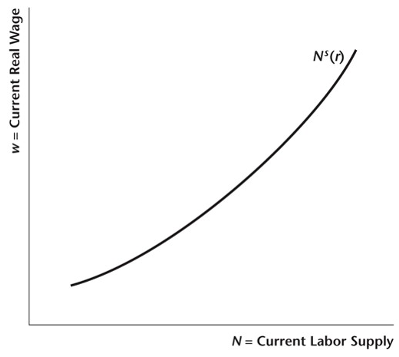
\includegraphics[scale=0.6]{Figures/W_Fig_11pt1.png}
\end{figure}
\end{frame}


\begin{frame}
\frametitle[alignment=center]{Increase in the Real Interest Rate Shifts the Current Labor Supply Curve to the Right}
\begin{figure}
\centering
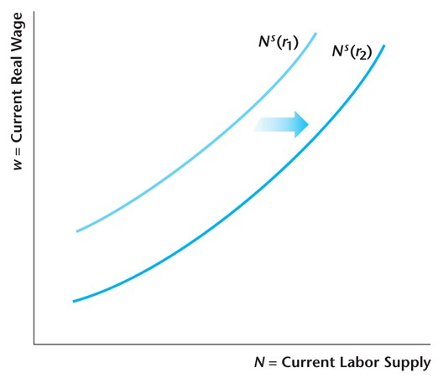
\includegraphics[scale=0.6]{Figures/W_Fig_11pt2.png}
\end{figure}
\end{frame}

\begin{frame}
\frametitle[alignment=center]{Increase in Lifetime Wealth Shifts the Current Labor Supply Curve to the Left}
\begin{figure}
\centering
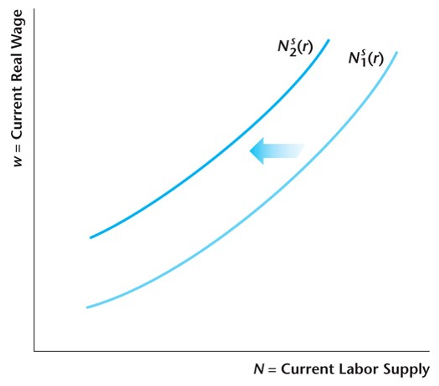
\includegraphics[scale=0.6]{Figures/W_Fig_11pt3.png}
\end{figure}
\end{frame}

\begin{frame}
\frametitle[alignment=center]{Current Demand for Consumption Goods}
$$MRS_{\ell,C}=w$$
\begin{itemize}
\item Similarly for consumption:
\begin{enumerate}
\item As current (total) income increases, consumption today increases
\item When real interest increase, consumption demand shifts down (assuming again income effect is muted)
\item When lifetime wealth increases, consumption demand shifts up
\end{enumerate}
\item With these we can graph out the labor supply curve and shifts
\end{itemize}
\end{frame}

\begin{frame}
\frametitle[alignment=center]{Consumption Today Increases as Current Income Increases}
\begin{figure}
\centering
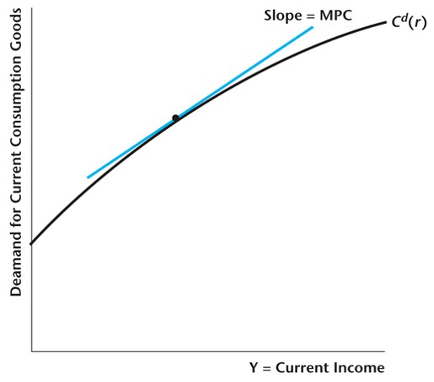
\includegraphics[scale=0.6]{Figures/W_Fig_11pt4.png}
\end{figure}
\end{frame}

\begin{frame}
\frametitle[alignment=center]{Consumption Today Decreases as Interest Rates Increase}
\begin{figure}
\centering
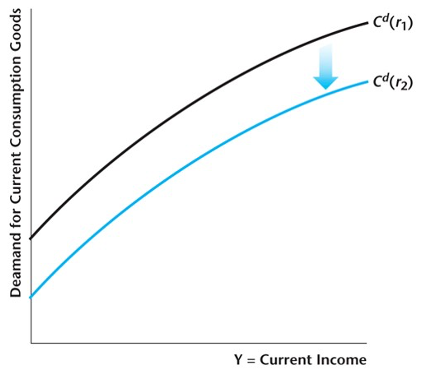
\includegraphics[scale=0.6]{Figures/W_Fig_11pt5.png}
\end{figure}
\end{frame}

\begin{frame}
\frametitle[alignment=center]{Consumption Today Increases as Lifetime Income Increases}
\begin{figure}
\centering
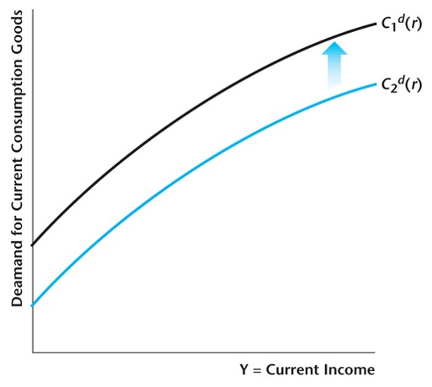
\includegraphics[scale=0.6]{Figures/W_Fig_11pt6.png}
\end{figure}
\end{frame}

\begin{frame}
\frametitle[alignment=center]{The Representative Firm}
\begin{itemize}
\item We have the consumer, now let's get the firm.  Production function(s):
$$Y=zF(K,N)\ \ \ \ Y'=z'F(K',N')$$
\item Law of motion of capital:
$$K'=(1-\delta)K+I$$
\item Firm profits:
$$\pi=Y-wN-I$$
$$\pi'=Y'-w'N'-(1-\delta)K'$$
\item Firm maximizes NPV of profits:
$$V=\pi+\frac{\pi'}{1+r}$$
\item Hires labor until $MP_N=w$
\end{itemize}
\end{frame}

\begin{frame}
\frametitle[alignment=center]{The Demand Curve for Current Labor is the Representative Firm's Marginal Product of Labor Schedule}
\begin{figure}
\centering
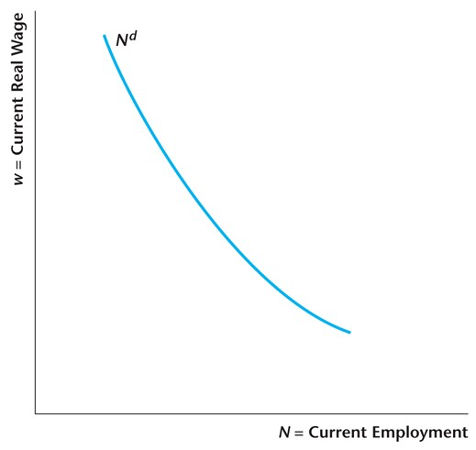
\includegraphics[scale=0.6]{Figures/W_Fig_11pt7.png}
\end{figure}
\end{frame}

\begin{frame}
\frametitle[alignment=center]{The Demand Curve for Current Labor Shifts Out with TFP}
\begin{figure}
\centering
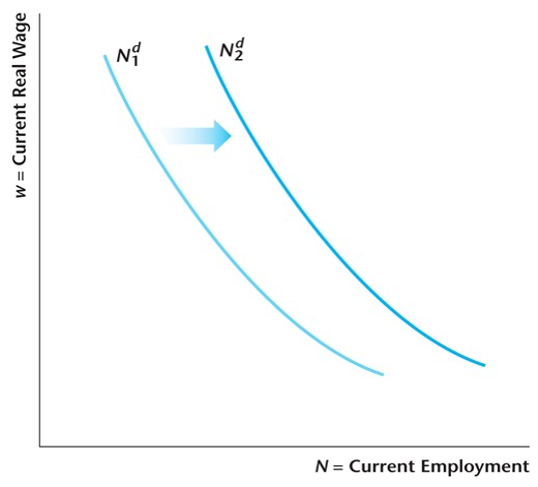
\includegraphics[scale=0.6]{Figures/W_Fig_11pt8.png}
\end{figure}
\end{frame}

\begin{frame}
\frametitle[alignment=center]{The Representative Firm-Investment}
\begin{itemize}
\item Marginal cost of investment is just one (numeraire) $MC(I)=1$
\bigskip
\item Marginal benefit of investment is complicated--discounted MPK of tomorrow for whatever's left:
$$MB(I)=\frac{MP_K'+1-\delta}{1+r}$$
\item Which gives:
$$MP_K'=r+\delta$$
\item Optimal investment rule:  the real interest rate (including depreciation) should equal the marginal product of capital
\bigskip
\item We could also have gotten this if households had loaned out the capital
\bigskip
\item Optimal investment schedule:
\begin{itemize}
\item Shifts to right when future TFP $z'$ increases
\item Shifts to left when current capital stock $K$ is higher 
\end{itemize}
\end{itemize}
\end{frame}

\begin{frame}
\frametitle[alignment=center]{As the real interest rates falls, quantity of investment demanded rises}
\begin{figure}
\centering
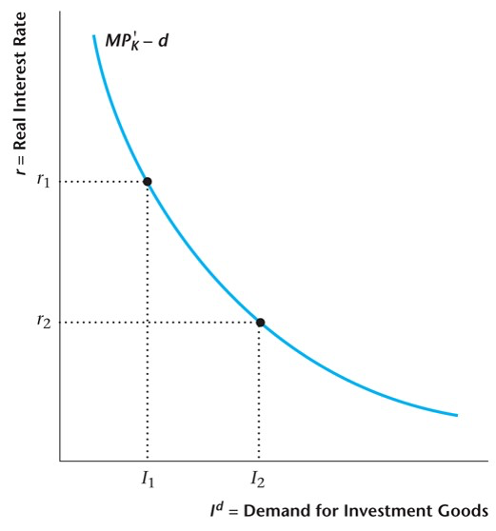
\includegraphics[scale=0.6]{Figures/W_Fig_11pt9.png}
\end{figure}
\end{frame}

\begin{frame}
\frametitle[alignment=center]{As TFP increases, investment demand rises}
\begin{figure}
\centering
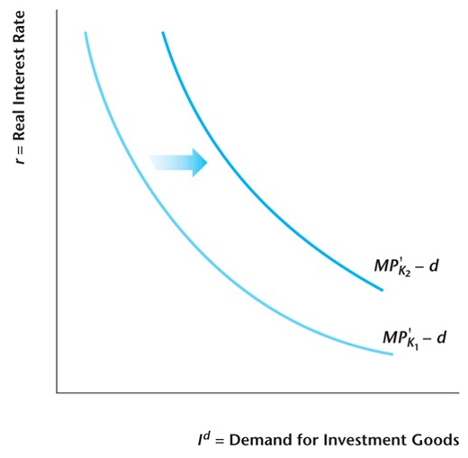
\includegraphics[scale=0.6]{Figures/W_Fig_11pt10.png}
\end{figure}
\end{frame}

\begin{frame}
\frametitle[alignment=center]{Investing with Asymmetric Information}
\begin{itemize}
\item We assumed perfect capital markets before
\bigskip
\item But in reality, some firms may be ``riskier" and the risk premium on their loans may change over the business cycle
\bigskip
\item Let $r$ be the ``safe" interest rate and $r^l$ be a loan interest rate.
\bigskip
\item Now the investment decision becomes:
$$MP_K'-\delta=r+x$$
\item This shifts up MPK, which shifts down investment
\end{itemize}
\end{frame}

\begin{frame}
\frametitle[alignment=center]{The Effect of an Increased Default Premium on a Firm's Optimal Investment Schedule}
\begin{figure}
\centering
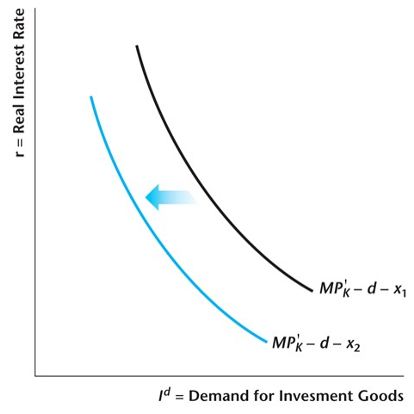
\includegraphics[scale=0.6]{Figures/W_Fig_11pt11.png}
\end{figure}
\end{frame}

\begin{frame}
\frametitle[alignment=center]{Investment and the Interest Rate Spread}
\begin{figure}
\centering
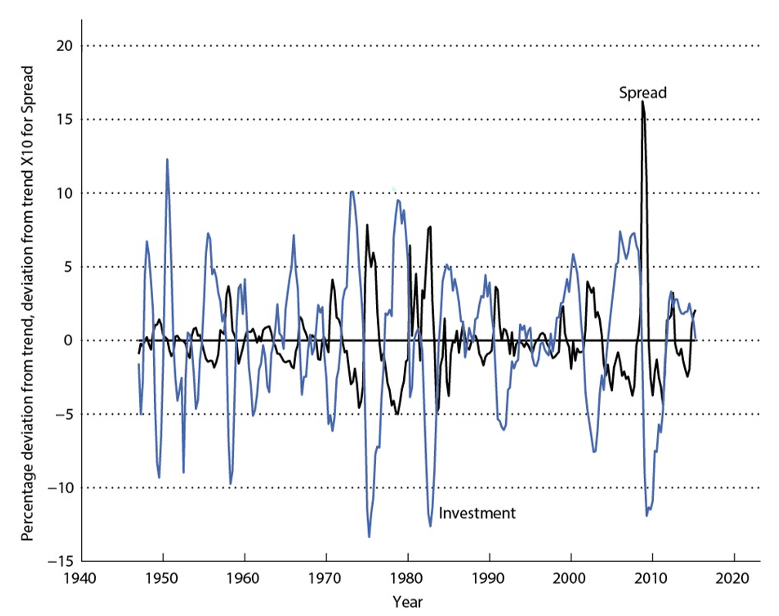
\includegraphics[scale=0.6]{Figures/W_Fig_11pt12.png}
\end{figure}
\end{frame}

\begin{frame}
\frametitle[alignment=center]{Scatter Plot: Investment vs Interest Rate Spread}
\begin{figure}
\centering
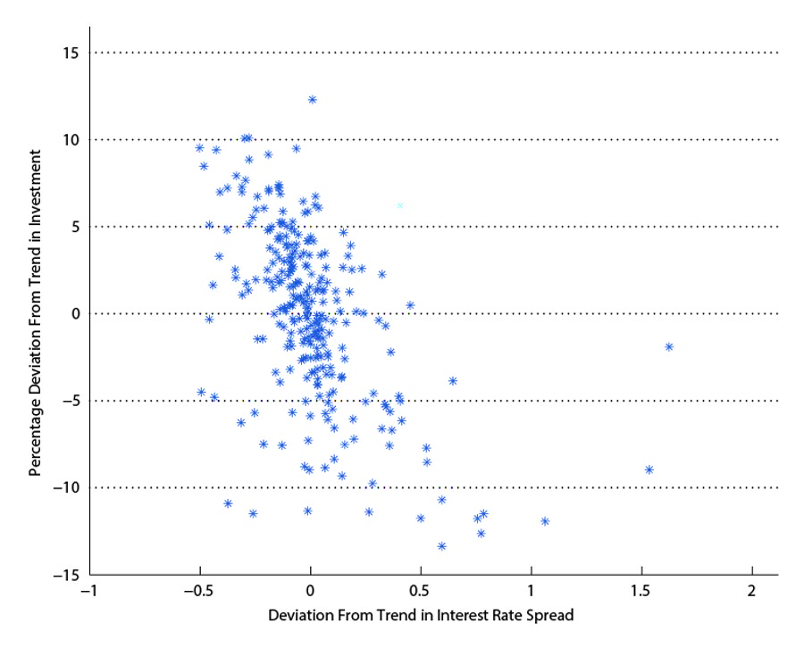
\includegraphics[scale=0.6]{Figures/W_Fig_11pt13.png}
\end{figure}
\end{frame}


\begin{frame}
\frametitle[alignment=center]{Government}
\begin{itemize}
\item Government is as it was before:
$$G+\frac{G'}{1+r}=T+\frac{T'}{1+r}$$
\end{itemize}
\end{frame}



\begin{frame}
\frametitle[alignment=center]{Competitive Equilibrium}
\begin{itemize}
\item We have a:
\begin{itemize}
\item Representative consumer that works, leisures, consumes, saves, and pays taxes
\bigskip
\item We have firms that take in labor, invest in capital, and produce
\bigskip
\item We have a government that taxes and spends
\end{itemize}
\item Thus far, we ignore future markets in labor and goods, though they obviously would affect a consumer/worker/firm today!
\bigskip
\item This won't change most of our qualitative results
\bigskip
\item Equilibrium will be when supply=demand, budget constraints hold, and agents optimize
\end{itemize}
\end{frame}

\begin{frame}
\frametitle[alignment=center]{Determination of Equilibrium in the Labor Market Given the Real Interest Rate $r$}
\begin{figure}
\centering
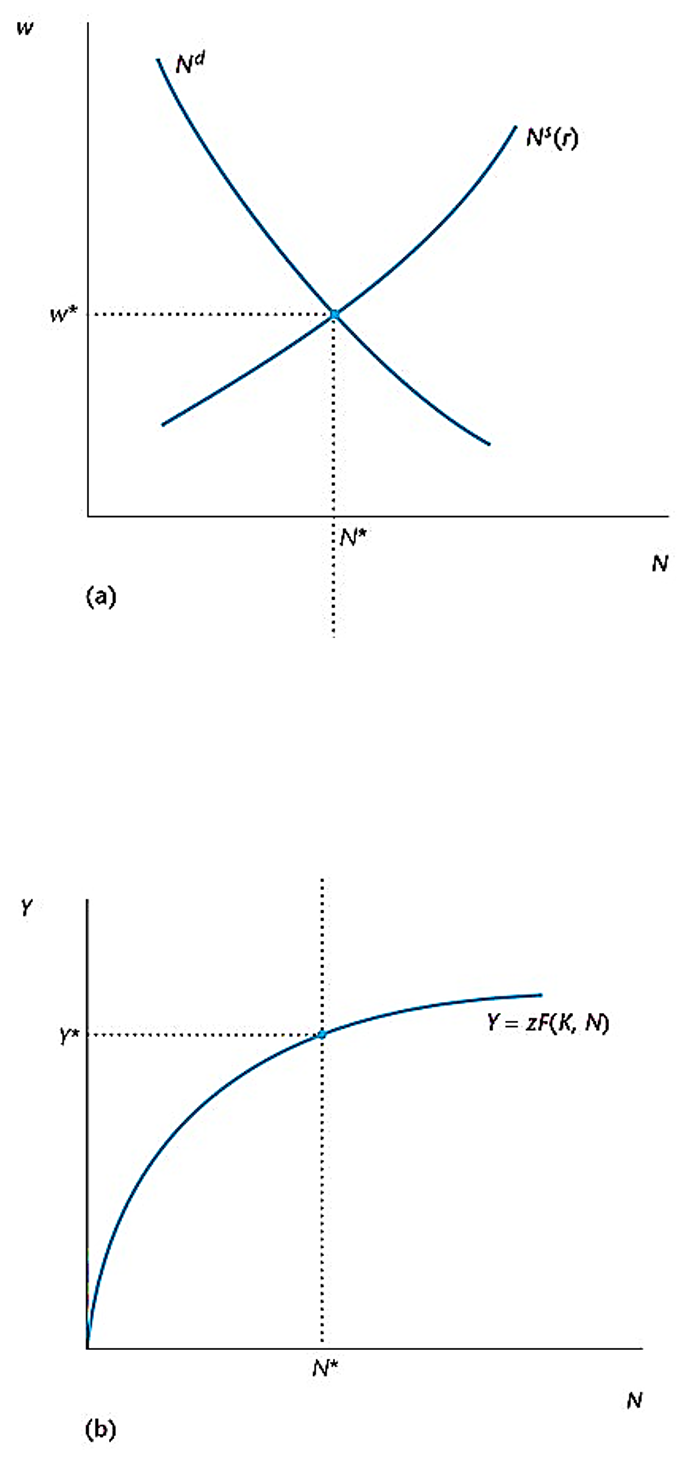
\includegraphics[scale=0.6]{Figures/W_Fig_11pt14.png}
\end{figure}
Given $r$ and $w$, we have labor supply \& demand, and wage. Given labor, we have production.  
\end{frame}

\begin{frame}
\frametitle[alignment=center]{Construction of the Output Supply Curve $Y(r)$} 
\begin{figure}
\centering
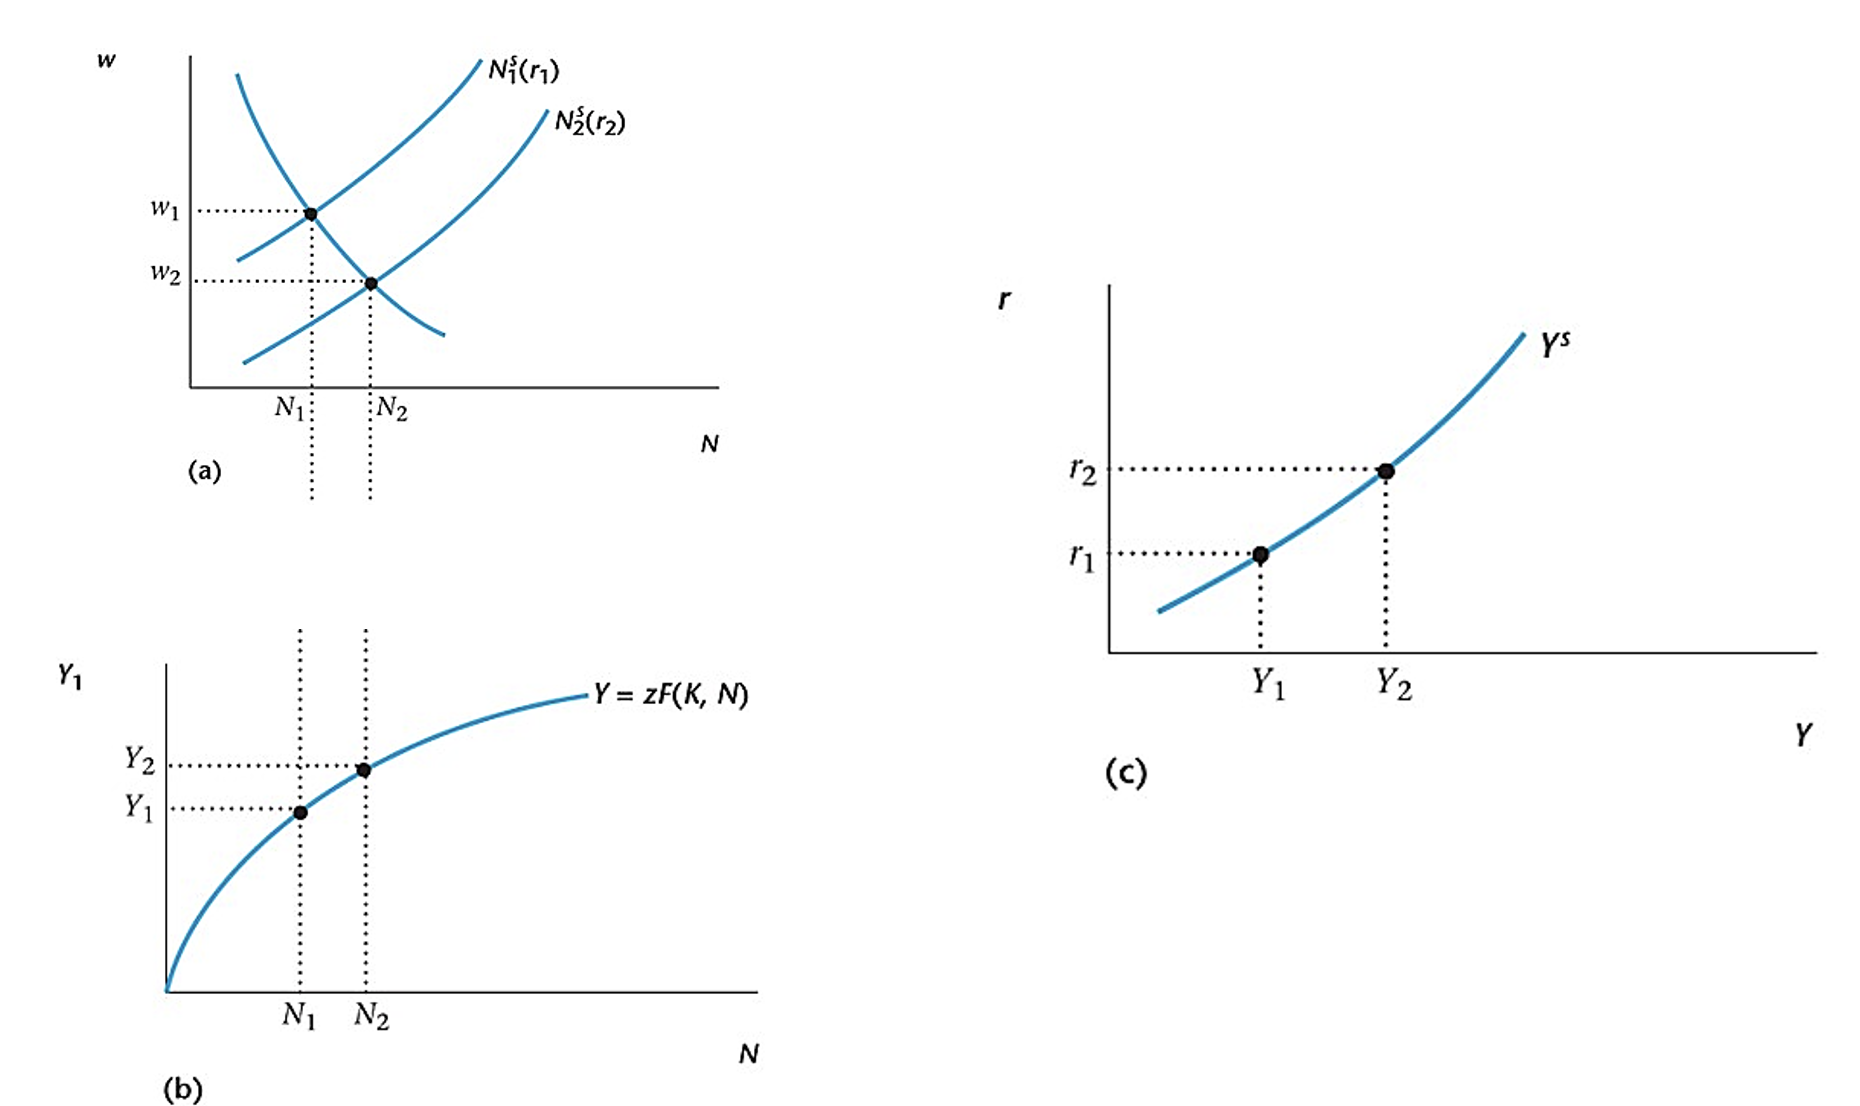
\includegraphics[scale=0.3]{Figures/W_Fig_11pt15.png}
\end{figure}
We can trace out how shifts in $r$ affect $Y$.  
\end{frame}

\begin{frame}
\frametitle[alignment=center]{What shifts the output supply curve?}
\begin{itemize}
\item Increase in lifetime wealth (such as from a decrease in government taxation) shifts the labor supply in, which causes the output supply curve to shift down
\bigskip
\item Current total factor productivity increase shifts the labor demand out, which causes the output supply curve to shift up 
\bigskip
\item Current capital stock increase shifts the labor demand out, which causes the output supply curve to shift up 
\end{itemize} 
\end{frame}


\begin{frame}
\frametitle[alignment=center]{An Increase in Current or Future Government Spending Shifts the $Y^S$ Curve} 
\begin{figure}
\centering
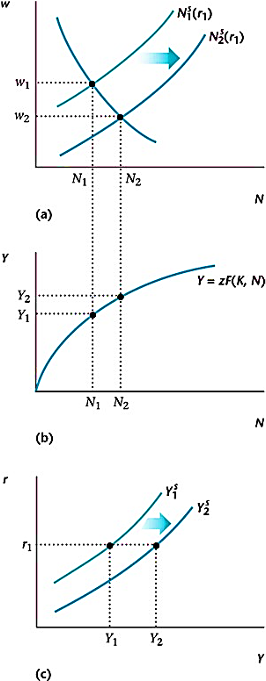
\includegraphics[scale=0.62]{Figures/W_Fig_11pt16.png}
\end{figure}
We can trace out how shifts in $r$ affect $Y$.  
\end{frame}

\begin{frame}
\frametitle[alignment=center]{Shifting to Demand} 
\begin{itemize}
\item Now we have the output supply curve, and how it reacts to changes in interest rates and government expenditure, we need the output demand curve
\bigskip
\item Decreases in taxes shifts $Y^D$ to the right (lifetime wealth increases)
\bigskip
\item  Increase in future income $Y'$ shifts $Y^D$ to the right (lifetime wealth increases)
\bigskip
\item Increase in future TFP shifts $Y^D$ to the right (lifetime wealth increases)
\bigskip
\item Decrease in current capital stock shifts $Y^D$ to the right (more demand for capital)
\end{itemize}
\end{frame}

\begin{frame}
\frametitle[alignment=center]{Output Demand} 
\begin{figure}
\centering
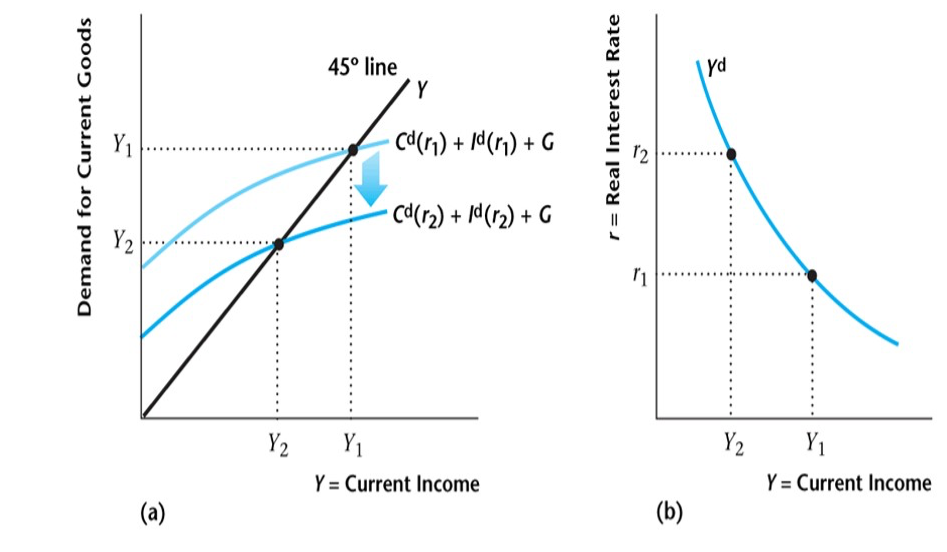
\includegraphics[scale=0.55]{Figures/W_Fig_11pt19.png}
\end{figure}
\end{frame}

\begin{frame}
\frametitle[alignment=center]{Putting it All Together} 
\begin{itemize}
\item We have output demand and supply
\bigskip
\item Labor market clear via wages
\bigskip
\item Output market clears via interest rates
\bigskip
\item Putting them together graphically
\end{itemize}
\end{frame}

\begin{frame}
\frametitle[alignment=center]{Equilibrium in a Real Intertemporal Model} 
\begin{figure}
\centering
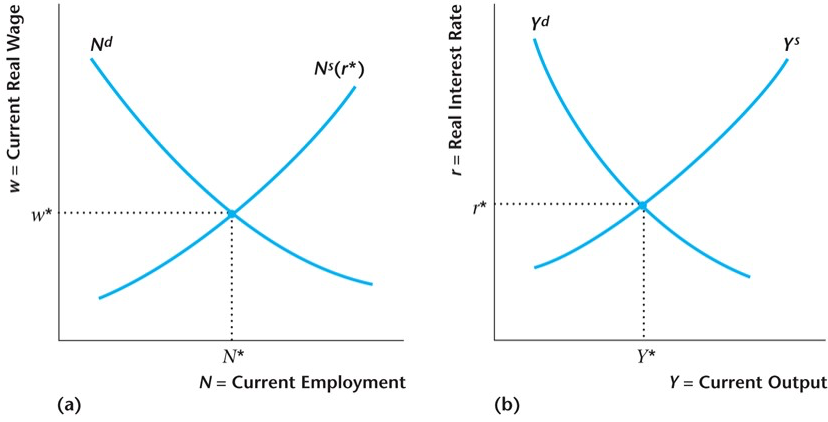
\includegraphics[scale=0.52]{Figures/W_Fig_11pt21.png}
\end{figure}
Now we can start analyzing various policies!
\end{frame}

\begin{frame}
\frametitle[alignment=center]{Policies} 
\begin{itemize}
\item Now that we have a real dynamic equilibrium model, we can use it to analyze various policies:
\begin{enumerate}
\item How does an increase in current government purchases, anticipated to be temporary, affect current macroeconomic variables?
\item What are the effects on current macroeconomic variables of a decrease in the current capital stock, brought about by a natural disaster or a war?
\item How does a temporary increase in total factor productivity affect macroeconomic variables, and how does this fit the key business cycle facts?
\item If total factor productivity is expected to increase in the future, how does this affect current macroeconomic variables?
\item How do credit frictions affect macroeconomic activity?
\item What are the effects of sectoral shocks on the economy?
\end{enumerate}
\item Let's go through one by one!
\end{itemize}
\end{frame}

\begin{frame}
\frametitle[alignment=center]{Example 1: Temporary Increase in Government Purchases} 
\begin{itemize}
\item We did this before in our one-period model and found $G$  crowded out $C$
\bigskip
\item But now we're intertemporal!  We have an interest rate.  Three new things to examine:
\bigskip
\item As $G$ increases, it will increase the interest rate, which will affect both investment and consumption
\bigskip
\item As $G$ increases, labor supply will be intertemporally substituted 
\bigskip
\item Now we have government spending multipliers!
\end{itemize}
\end{frame}

\begin{frame}
\frametitle[alignment=center]{Temporary Increase in Government Purchases} 
\begin{itemize}
\item When current period $G$ shifts from $G_1$ to $G_2$, we need to know the change in output demand
\bigskip
\item We will assume that MPC is a constant, and denote the shift in the output demand curve as $\Delta$, so that:
$$\Delta=G_2-G_1-MPC(G_2-G_1)+MPC\Delta$$
\item Where:
\begin{itemize}
\item  $G_2-G_1$ is the direct effect of an increase in government expenditure on goods demanded
\item $MPC(G_2-G_1)$ is the effect of an increase in taxes on consumer expenditure (crowd-out)
\item $MPC\Delta$ is the add-on effect of an increase in wealth on consumer expenditure
\end{itemize}
\item Solving for $\Delta$, we get $\Delta=1$
\item And the demand multiplier $m_d=\frac{\Delta}{G_2-G_1}=1$
\item But now need affects on $w$, $N$, $r$, $Y$
\end{itemize}
\end{frame}

\begin{frame}
\frametitle[alignment=center]{Temporary Increase in Government Purchases} 
\begin{itemize}
\item $G$ increases from $G_1$ to $G_2$
\item $Y^D$ shifts one-for-one with increase in expenditures
\item Lifetime wealth decreases, so demand for leisure decreases, labor supply increases
\item When labor supply increases, output supply increases
\item Output supply typically shifts by less than output demand (small effect on wealth), so interest rates increase
\item When interest rates increase, labor supply increases further
\item Let's see it graphically
\end{itemize}
\end{frame}


\begin{frame}
\frametitle[alignment=center]{Example 1: Increase in Govt Purchases} 
\begin{figure}
\centering
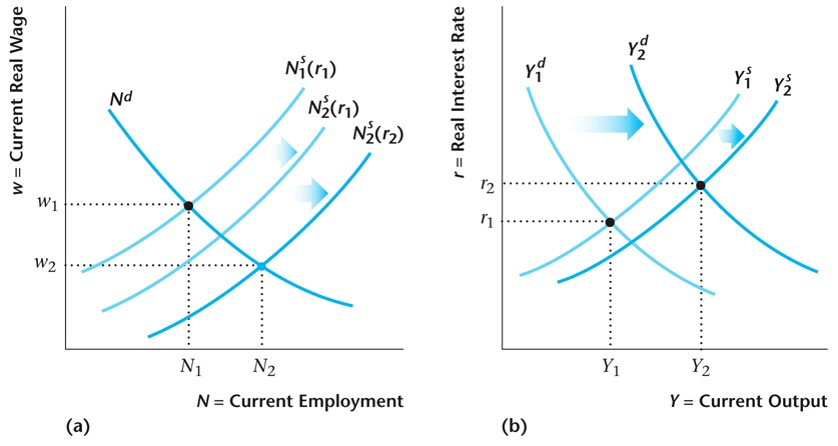
\includegraphics[scale=0.52]{Figures/W_Fig_11pt22.png}
\end{figure}
\end{frame}

\begin{frame}
\frametitle[alignment=center]{Government Expenditure Multiplier} 
\begin{itemize}
\item Total output shifts by less than the government's expenditure shift, as interest rates rise
\bigskip
\item Consequently the expenditure multiplier is less than one.
\bigskip
\item Multiplier is smaller if affect on labor supply via wealth decreases and interest rate increases are smaller
\bigskip
\item Some argue its more than one!  We'll tackle these models later, but we can see graphically that if interest rates didn't increase, 
\bigskip
\item For now, let's move to the effects of a decrease in capital stock $K$
\end{itemize}
\end{frame}


\begin{frame}
\frametitle[alignment=center]{Example 2: Decrease in $K$} 
\begin{itemize}
\item Now let's say that $K$ shifts from $K_1$ to $K_2$, $K_2<K_1$
\bigskip
\item Firms are less productive, so demand for labor shifts downwards, and output supply shifts downwards
\bigskip
\item Capital is in short supply, so output demand shifts outwards
\bigskip
\item We see that both push up the interest rate $r$, but the affects on output are unclear
\bigskip
\item As $r$ increases, labor supply shifts out
\bigskip
\item Workers are less productive, so $w$ falls, but what happens to employment is similarly unclear
\end{itemize}
\end{frame}


\begin{frame} 
\frametitle[alignment=center]{Decrease in Capital} 
\begin{figure}
\centering
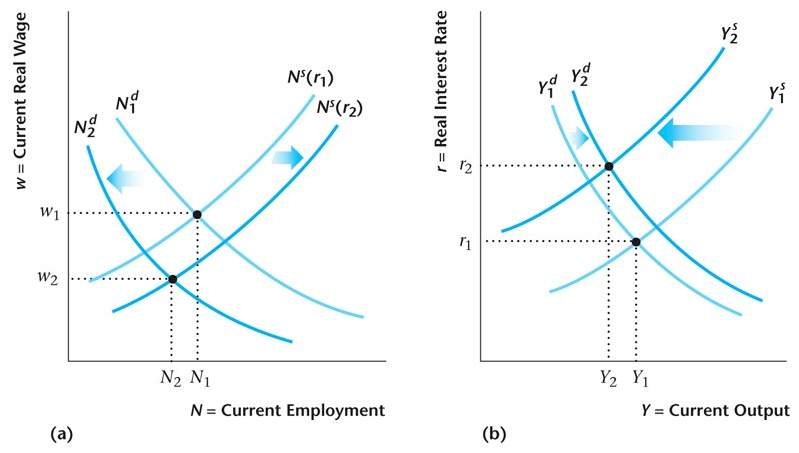
\includegraphics[scale=0.52]{Figures/W_Fig_11pt24.png}
\end{figure}
\end{frame}

\begin{frame}
\frametitle[alignment=center]{Example 3: Increase in current TFP $z$} 
\begin{itemize}
\item Now let's say that $z$ shifts from  $z_1$ to $z_2$, $z_2>z_1$
\bigskip
\item Firms are more productive, so demand for labor shifts outwards, and output supply shifts outwards
\bigskip
\item Interest rates fall as output shifts out, so supply of labor shifts in slightly
\bigskip
\item Because the shift in labor demand dominates, wages rise and labor increases
\bigskip
\item Importantly, consumption, real wages, investment, employment, and average labor productivity all move together, which is what we saw in the data
\end{itemize}
\end{frame}

\begin{frame} 
\frametitle[alignment=center]{Decrease in Capital} 
\begin{figure}
\centering
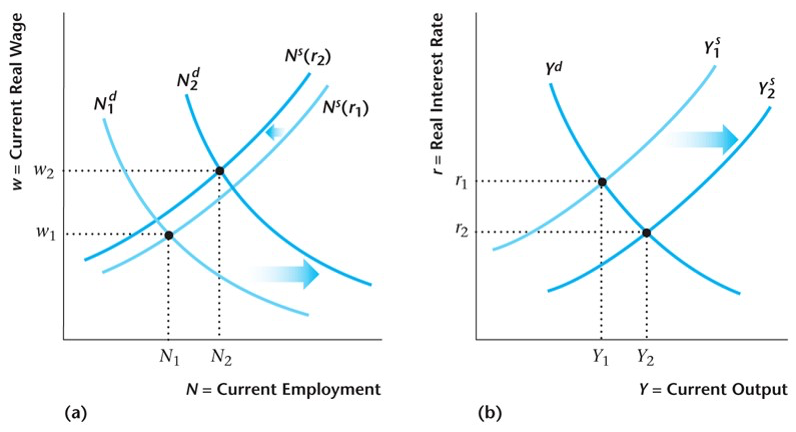
\includegraphics[scale=0.52]{Figures/W_Fig_11pt25.png}
\end{figure}
\end{frame}



\begin{frame}
\frametitle[alignment=center]{Example 4: Increase in future TFP $z'$} 
\begin{itemize}
\item Now let's say that $z'$ shifts from  $z_1'$ to $z_2'$, $z_2'>z_1'$
\bigskip
\item Firms know future $MPK$ is higher, so demand for investment increases, output demand increases
\bigskip
\item This causes interest rates to rise, increasing labor supply, driving wages down and labor up
\end{itemize}
\end{frame}

\begin{frame} 
\frametitle[alignment=center]{Increase in Future TFP} 
\begin{figure}
\centering
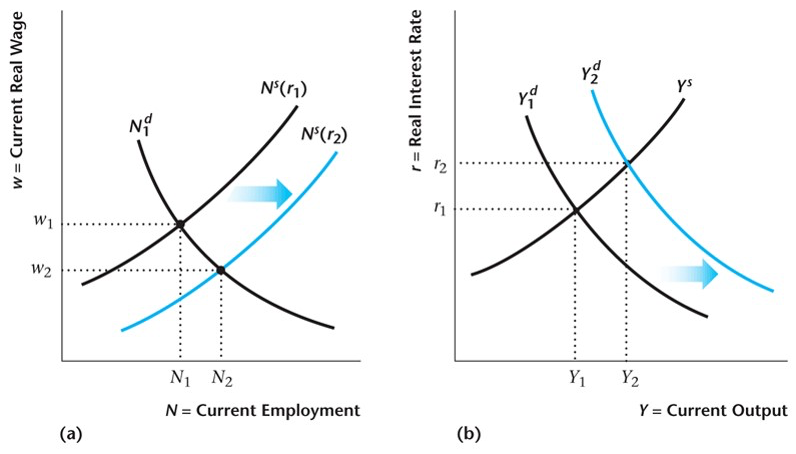
\includegraphics[scale=0.52]{Figures/W_Fig_11pt27.png}
\end{figure}
\end{frame}


\begin{frame}
\frametitle[alignment=center]{Example 5: Credit Frictions} 
\begin{itemize}
\item Credit frictions, due to asymmetric information and limited commitment, operate through the interest rate
\bigskip
\item $r$ increases due to wedge/risks, lowering output demand and increasing labor supply
\bigskip
\item As labor supply increases, output supply increases
\bigskip
\item Output could rise or fall--in practice, the effect on consumption falling is larger than the effect on labor, so output falls
\bigskip
\item When it falls, labor demand falls
\end{itemize}
\end{frame}

\begin{frame} 
\frametitle[alignment=center]{Increase in Credit Frictions} 
\begin{figure}
\centering
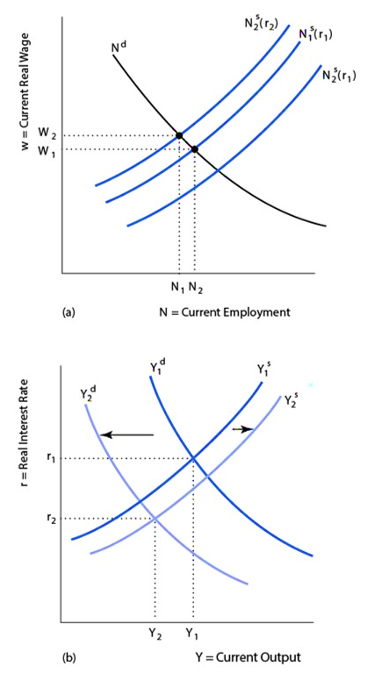
\includegraphics[scale=0.58]{Figures/W_Fig_11pt29.png}
\end{figure}
\end{frame}

\begin{frame}
\frametitle[alignment=center]{Example 6: Sectoral Shocks} 
\begin{itemize}
\item Sectoral shocks are disturbances to technology and preferences
\bigskip
\item Idea is that the market is reallocating resources and experiencing ``mismatch"
\bigskip
\item We'll model a shock tat affects labor market mismatch--acts as a friction, so workers and firms both experience an extra non-market cost to matching (like a tax wedge!)
\bigskip
\item Labor demand and supply shift down, so output supply shifts down
\bigskip
\item This increases MPL/average labor productivity 
\end{itemize}
\end{frame}

\begin{frame} 
\frametitle[alignment=center]{Sectoral Shock/Mismatch} 
\begin{figure}
\centering
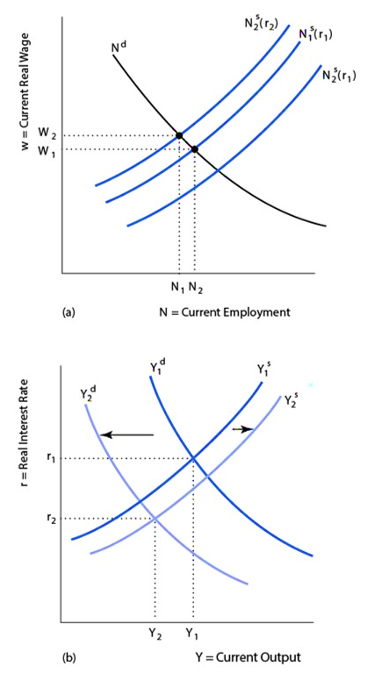
\includegraphics[scale=0.54]{Figures/W_Fig_11pt29.png}
\end{figure}
\end{frame}



\begin{frame} 
\frametitle[alignment=center]{Summary} 
\begin{itemize}
\item We have a real, dynamic (two-period) model of the macroeconomy
\bigskip
\item  Lets us think about investment, consumption, output, real interest rates, and employment
\bigskip
\item Two (linked) key markets we think through:  labor supply/demand, and output supply/demand
\bigskip
\item Interest rates clear output markets, and affect labor supply
\bigskip
\item Can think through a variety of examples cleanly
\end{itemize}
\end{frame}



\end{document}